\chapter{Investigación}

	\section{ADCs}
	
	
	\section{DACs}
	

    En este capitulo se presentan los conceptos necesarios para comprender cómo funcionan las diferentes clases de generadores de números aleatorios, sus fuentes de aleatoriedad, sus principales características y cuales son factibles para implementación en FPGA.


El jitter del reloj en un sistema digital es una desviación del flanco de reloj real con respecto a un flanco de reloj ideal. Una señal de reloj ideal se define mediante la ecuación (\ref{eq:señal_periodica}), donde $t(n)$ representa el tiempo del periodo $n$-ésimo de una señal de reloj y $T$ es el periodo de una señal de reloj.

            \begin{equation}
                t(n) = n \cdot T 
                \label{eq:señal_periodica}
            \end{equation}
            
            En la práctica, una señal de reloj real no alcanza siempre múltiplos enteros de su periodo ideal, sino que sus flancos fluctúan alrededor de este valor debido al jitter. Esta variación es causada por diversos fenómenos físicos, como el ruido térmico, el ruido de la fuente de alimentación y el ruido electromagnético ambiental, entre otros. La Figura \ref{fig:F9_jitter} muestra cómo se ve una señal de reloj afectada por el jitter.

            \begin{figure}[hbtp]
                \centering
                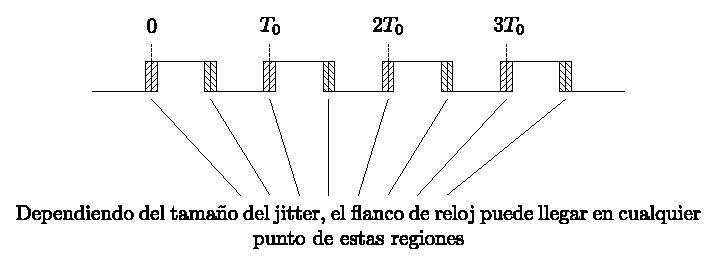
\includegraphics[width=0.8\textwidth]{F9_jitter}
                \caption{Jitter del reloj.}
                \label{fig:F9_jitter}
            \end{figure}
            
            
            Los parámetros recomendados para configurar las pruebas NIST se muestran en la Tabla \ref{tab:NIST_parametros}:

            \begin{table}[htbp]
                \caption{Parámetros recomendados para el conjunto de pruebas del NIST.}
                \begin{center}
                    \resizebox{0.8\linewidth}{!}{ 
                    \begin{NiceTabular}{|l|l|l|}
                        \CodeBefore
                        \rowcolor{lightgray}{1}
                        \Body
                        \hline
                        \textbf{Test}  & \textbf{Configuration item} & \textbf{Setting} \\
                        \hline
                        All tests   & Bits per sequence & 1000000  \\
                        \hline
                        All test   & Number of sequences (sample size) & 1073 \\
                        \hline
                        Frequency test within a block & Block length & 20000  \\
                        \hline
                        Non-overlapping template test  & Template length & 10  \\
                        \hline
                        Overlapping template & Block length & 10 \\
                        \hline
                        Mauler's Universal Statistical test  & Test block length L &  7 \\
                        \hline
                        Mauler's Universal Statistical test  & Initialization steps  &  1280 \\
                        \hline
                        Approximate entropy test & Block length &  8 \\
                        \hline
                        Linear complexity test  & Block length &  1000 \\
                        \hline
                        Serial test & Block length &  16 \\
                        \hline
                    \end{NiceTabular}
                    }
                \label{tab:NIST_parametros}
                \end{center}
            \end{table}